%tag:000X
%label:"dig:symplecticCohomologyTelescope"
%type:"diagram"
%parent:con:symplecticCohomologyLimit
%author:JeffHicks

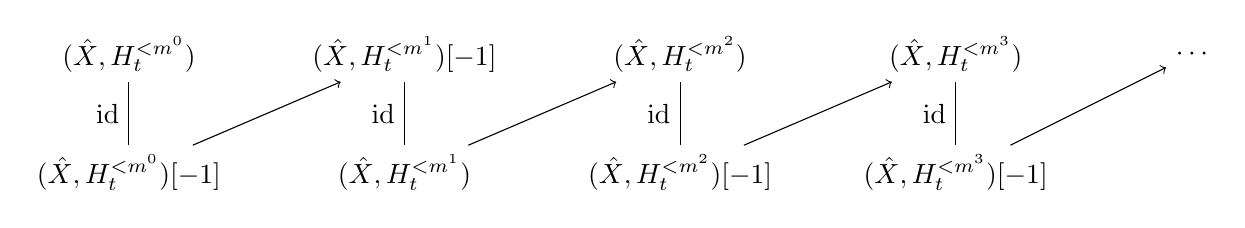
\begin{tikzpicture}
    \node (v1) at (-15,-2.5) {$\CF(\hat X, H_t^{<m^0})[-1]$};
    \node (v2) at (-15,-1) {$\CF(\hat X, H_t^{<m^0})$};
    \node (v4) at (-11.5,-1) {$\CF(\hat X, H_t^{<m^1})[-1]$};
    \node (v3) at (-11.5,-2.5) {$\CF(\hat X, H_t^{<m^1})$};
    \node (v5) at (-8,-2.5) {$\CF(\hat X, H_t^{<m^2})[-1]$};
    \node (v6) at (-8,-1) {$\CF(\hat X, H_t^{<m^2})$};
    \node (v8) at (-4.5,-1) {$\CF(\hat X, H_t^{<m^3})$};
    \node (v7) at (-4.5,-2.5) {$\CF(\hat X, H_t^{<m^3})[-1]$};
    \node (v9) at (-1.5,-1) {$\cdots$};
    \draw  (v1) edge node[left]{id} (v2);
    \draw  (v3) edge node[left]{id}  (v4);
    \draw  (v5) edge node[left]{id} (v6);
    \draw  (v7) edge node[left]{id}  (v8);
    \draw  (v1) edge[->] (v4);
    \draw  (v3) edge[->] (v6);
    \draw  (v5) edge[->] (v8);
    \draw (v7) edge[->] (v9);
\end{tikzpicture}